\documentclass[addpoints,12pt]{exam}
%\usepackage[fontsize=18pt]{scrextend}
\newcommand{\ds}{\displaystyle}
\usepackage[margin=0.8in]{geometry}
\usepackage{subcaption}
\usepackage{pgfplots}
\usepackage{multicol}
\pgfplotsset{compat=1.16}

\usepackage{amssymb,amsmath,graphicx,wrapfig,verbatim, psfragx,color}
\usepackage{multicol}
\usepackage{wasysym}
\usepackage{tikz}
\usetikzlibrary{fit}
\usetikzlibrary{shapes}
\usetikzlibrary{calc}
\usetikzlibrary{3d}
\pgfplotsset{my style/.append style={axis x line=middle, axis y line=
middle, xlabel={$x$}, ylabel={$y$}, axis equal }}



% If you want them as a list (instead of next to each other)
\usepackage{enumitem}

% ---- Convenience commands -----

% Choose one option (bubbles)
\newcommand{\chooseone}{{\Large$\Circle$\ \ }}

% ---- Example Usage | Multiple Choice -----


%\usepackage{fancyhdr}
%\setlength{\headheight}{13.6pt}
%\pagestyle{fancy}
%\lhead{Math 222}
%\chead{ Midterm 1 }
%\rhead{Spring 2022}

\NewDocumentEnvironment{QBoxes}{ +b }{%
    \checkboxchar{\(\Box\)}
    \begin{checkboxes}
        #1
    \end{checkboxes}
}

\def\FillInBlank{\rule{3truein} {.01truein}}
\newcommand{\TorF}{\hspace{.1in} \textbf{True} \hspace{.1in} \textbf{False}  \hspace{.1in}}


\newcommand{\myleft}{\makebox[.4\textwidth]{First Name:\enspace\hrulefill}}
\newcommand{\myright}{\makebox[.4\textwidth]{Last Name:\enspace\hrulefill}}
\header{\oddeven{\myleft}{}}
       {}
       {\oddeven{\myright}{}}

\footrule

\footer{Math 112}
       {Midterm 1 - 
       Spring 2025}
       %Fall 2025}
       {Page \thepage\ of \numpages}

\begin{document}
Multiple choice section. All points are for choosing the correct answer(s). No justification is needed.
\begin{questions} 

\question[3] %(Joey) 
 \textbf{Select ALL} of the following that are functions:% relations:
\begin{multicols}{2}
\checkboxchar{\Large$\Box$}\begin{checkboxes}


\choice \phantom{a}\vspace{-.7cm}

  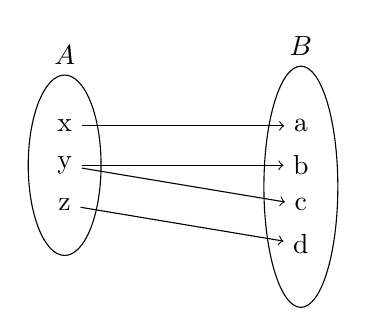
\begin{tikzpicture}
    \foreach[count=\i] \lseti/\lsetmi in {A/{x,y,z},B/{a,b,c,d}} {
        \begin{scope}[local bounding box=\lseti, x=3cm, y=.5cm]
        \foreach[count=\j] \lj in \lsetmi {
            \node[minimum width=1em] (n-\j-\lseti) at (\i,-\j) {\lj};
        }
        \end{scope}
        \node[ellipse, draw, fit=(\lseti), 
        label={[name=l-\lseti]above:$\lseti$}] {};
    }
    \draw[->] (n-1-A) -- (n-1-B);
    \draw[->] (n-2-A) -- (n-2-B);
   % \draw[->] (n-3-A) -- (n-1-B);
    \draw[->] (n-3-A) -- (n-4-B);
    \draw[->] (n-2-A) -- (n-3-B);
\end{tikzpicture}
\vfill
\choice \phantom{a}\vspace{-.7cm}

  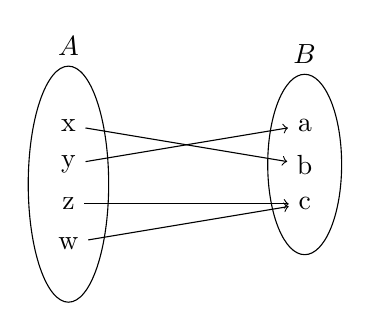
\begin{tikzpicture}
    \foreach[count=\i] \lseti/\lsetmi in {A/{x,y,z,w},B/{a,b,c}} {
        \begin{scope}[local bounding box=\lseti, x=3cm, y=.5cm]
        \foreach[count=\j] \lj in \lsetmi {
            \node[minimum width=1em] (n-\j-\lseti) at (\i,-\j) {\lj};
        }
        \end{scope}
        \node[ellipse, draw, fit=(\lseti), 
        label={[name=l-\lseti]above:$\lseti$}] {};
    }
    \draw[->] (n-1-A) -- (n-2-B);
    \draw[->] (n-2-A) -- (n-1-B);
   % \draw[->] (n-3-A) -- (n-1-B);
    \draw[->] (n-3-A) -- (n-3-B);
    \draw[->] (n-4-A) -- (n-3-B);
\end{tikzpicture}
%\vspace{1cm}
\choice
\phantom{a}\vspace{-.7cm}
    
    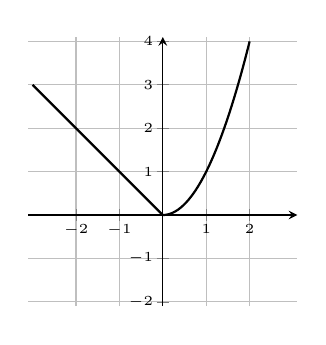
\begin{tikzpicture}%[domain=-4:4]
    \begin{axis}[
    grid=major,
    axis x line = middle,
    axis y line = middle,
        yticklabel style = {font=\tiny,xshift=0.5ex},
        xticklabel style = {font=\tiny,yshift=0.5ex},
    %scale only axis=true,
    width=5 cm,
    height=5 cm,
    xtick={-2,-1,0,1,2},
    ytick={-2,-1,0,1,2,3,4},
    xmin=-3.1,
    xmax=3.1,
    ymin=-2.1,
    ymax=4.1,
    ]
\addplot[smooth, thick, domain = 0:2,samples=35] { (x^2)};
\addplot[smooth, thick, domain = -3:0,samples=35] { -x};
  \end{axis}
\end{tikzpicture}

\vspace{.5cm}
\choice \phantom{a}\vspace{-.7cm}

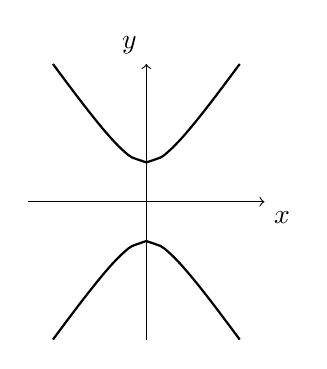
\begin{tikzpicture}[scale=.5]
    % Draw axes
    \draw[->] (-3, 0) -- (3, 0) node[anchor=north west] {$x$};
    \draw[->] (0, -3.5) -- (0, 3.5) node[anchor=south east] {$y$};
    

    
    % Draw the hyperbola branches (now vertically oriented)
    \draw[thick, smooth, domain=1:3.5, samples=20] plot ({sqrt((\x)^2/2 - .5)}, \x);
    \draw[thick, smooth, domain=1:3.5, samples=20] plot ({-sqrt((\x)^2/2 - .5)}, \x);
    \draw[thick, smooth, domain=-3.5:-1, samples=20] plot ({sqrt((\x)^2/2 - .5)}, \x);
    \draw[thick, smooth, domain=-3.5:-1, samples=20] plot ({-sqrt((\x)^2/2 - .5)}, \x);
    

\end{tikzpicture}

\end{checkboxes}
\end{multicols}
%\vfill

\question[3] Find the solution to the following inequality
\[|x-3|\ge-3\]
\begin{choices}
   \choice \chooseone $(-\infty,\infty)$
   \choice \chooseone $(-\infty,0]\cup[6,\infty)$
   \choice \chooseone There is no $x$ that solves the inequality.
   \choice \chooseone $[0,6]$
\end{choices}

\question[3] \textbf{Select ALL} (real and complex) solutions to the equation: 
\[x^3=-x \]
    \checkboxchar{\Large$\Box$}\begin{checkboxes}
        \choice $x=0$
        \choice $x=1$
        \choice $x=-1$
        \choice $x=i$   
        \choice $x=-i$
    \end{checkboxes}


\newpage

\question[3] Select the correct graph of $f(x)=\left\{\begin{matrix}
    x^2 &,& x\ge 0\\
    -x &,& x<0
\end{matrix}\right.$  
\begin{multicols}{2}
    

\begin{choices}
    \choice \chooseone\phantom{a}%\vspace{-.7cm}
    
    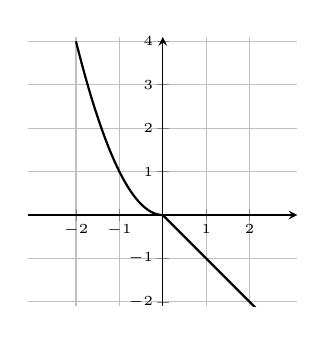
\begin{tikzpicture}%[domain=-4:4]
    \begin{axis}[
    grid=major,
    axis x line = middle,
    axis y line = middle,
        yticklabel style = {font=\tiny,xshift=0.5ex},
        xticklabel style = {font=\tiny,yshift=0.5ex},
    %scale only axis=true,
    width=5 cm,
    height=5 cm,
    xtick={-2,-1,0,1,2},
    ytick={-2,-1,0,1,2,3,4},
    xmin=-3.1,
    xmax=3.1,
    ymin=-2.1,
    ymax=4.1,
    ]
  %\draw[very thin,color=gray] (-2.9,-2.1) grid (2.9,2.9);
\addplot[smooth, thick, domain = -2:0,samples=35] { (x^2)};
\addplot[smooth, thick, domain = 0:3,samples=35] { -x};
  \end{axis}
\end{tikzpicture}

\choice \chooseone\phantom{a}%\vspace{-.7cm}
    
    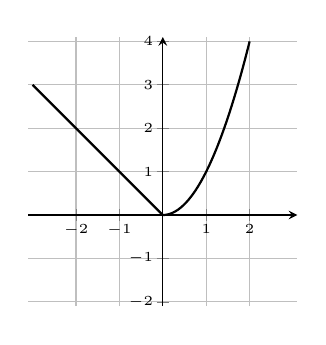
\begin{tikzpicture}%[domain=-4:4]
    \begin{axis}[
    grid=major,
    axis x line = middle,
    axis y line = middle,
        yticklabel style = {font=\tiny,xshift=0.5ex},
        xticklabel style = {font=\tiny,yshift=0.5ex},
    %scale only axis=true,
    width=5 cm,
    height=5 cm,
    xtick={-2,-1,0,1,2},
    ytick={-2,-1,0,1,2,3,4},
    xmin=-3.1,
    xmax=3.1,
    ymin=-2.1,
    ymax=4.1,
    ]
\addplot[smooth, thick, domain = 0:2,samples=35] { (x^2)};
\addplot[smooth, thick, domain = -3:0,samples=35] { -x};
  \end{axis}
\end{tikzpicture}

\choice \chooseone\phantom{a}%\vspace{-.7cm}
    
    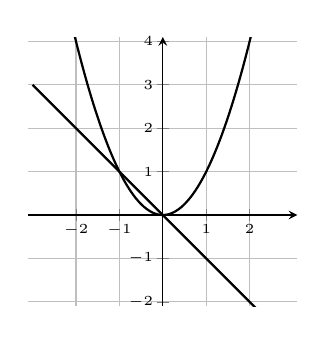
\begin{tikzpicture}%[domain=-4:4]
    \begin{axis}[
    grid=major,
    axis x line = middle,
    axis y line = middle,
        yticklabel style = {font=\tiny,xshift=0.5ex},
        xticklabel style = {font=\tiny,yshift=0.5ex},
    %scale only axis=true,
    width=5 cm,
    height=5 cm,
    xtick={-2,-1,0,1,2},
    ytick={-2,-1,0,1,2,3,4},
    xmin=-3.1,
    xmax=3.1,
    ymin=-2.1,
    ymax=4.1,
    ]
\addplot[smooth, thick, domain = -2.1:2.1,samples=35] { (x^2)};
\addplot[smooth, thick, domain = -3:3,samples=35] { -x};
  \end{axis}
\end{tikzpicture}
\choice \chooseone \phantom{a}%\vspace{-.7cm}
    
    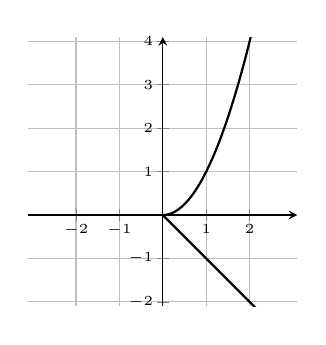
\begin{tikzpicture}
    \begin{axis}[
    grid=major,
    axis x line = middle,
    axis y line = middle,
        yticklabel style = {font=\tiny,xshift=0.5ex},
        xticklabel style = {font=\tiny,yshift=0.5ex},
    width=5 cm,
    height=5 cm,
    xtick={-2,-1,0,1,2},
    ytick={-2,-1,0,1,2,3,4},
    xmin=-3.1,
    xmax=3.1,
    ymin=-2.1,
    ymax=4.1,
    ]

\addplot[smooth, thick, domain = 0:2.1,samples=35] { (x^2)};
\addplot[smooth, thick, domain = 0:3,samples=35] { -x};
  \end{axis}
\end{tikzpicture}

\end{choices}
\end{multicols}

\question[3] If $f(x)=5x^2-\dfrac{1}{3-x}$, What is $f(-2z)$?
\begin{choices}
    \choice \chooseone $20z^2-\dfrac{1}{3+2z}$
    \choice \chooseone $-10z^3+\dfrac{2z}{3-z} $
    \choice \chooseone $-10z^3-\dfrac{2z}{3+2z}$
    \choice \chooseone $-20z^2+\dfrac{1}{3-2z}$
    \choice \chooseone None of the above.
\end{choices}

    \question[3] Find the domain of the function:
\[ \dfrac{\sqrt{x+3}}{x-7}\]
\begin{choices}
    \choice \chooseone $(-\infty, -3)\bigcup(-3,7)\bigcup(7,\infty)$
    \choice \chooseone $(-\infty, 7)\bigcup(7,\infty)$
    \choice \chooseone $[-3,7)\bigcup(7,\infty)$
    \choice \chooseone $[-3,\infty)$
    \choice \chooseone None of the Above.
\end{choices}

\newpage
\hspace{-.5in}Free answer section. Work must be shown to get credit for any answer. Partial credit may be given even for incorrect final answers, so show your work.

\question Given the graph of the function $y=F(x)$ describing the temperature of lake Mendota over one year below:
\begin{center}
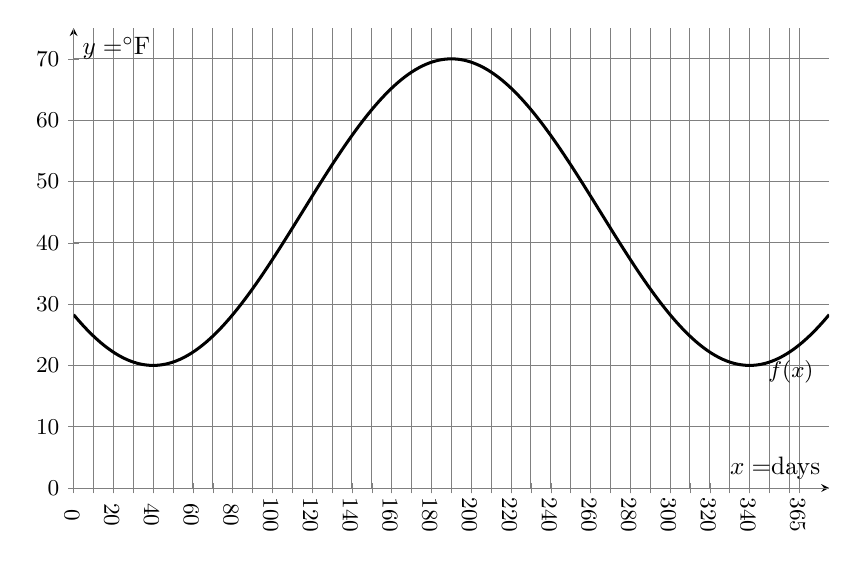
\begin{tikzpicture}[scale = .91]
    \begin{axis}[
        domain=0:380, % Defines the x range
        samples=200,  % Number of samples for smoothness
        width = \textwidth,
        height = 8cm,
        xlabel={$x=$days},
        ylabel={$y= ^\circ$F},
        axis lines=middle,
        grid=major, % Show only the main grid by default
        major grid style={solid, gray}, % Style for the main grid lines
        minor grid style={solid, lightgray}, % Style for the subgrid (lighter grey)
        xmin=0, xmax=380,  % Sets x-axis range
        ymin=0, ymax=75,  % Sets y-axis range
        xtick={0, 20, 40,60, 80, 100,120, 140,160, 180, 200,220, 240,260, 280, 300,320, 340,  365}, % Main ticks for x-axis
        ytick={0, 10, 20, 30, 40, 50, 60, 70}, % Main ticks for y-axis
        extra y ticks = {0},
        extra x ticks={0, 10,20,...,360}, % Subgrid ticks for x-axis
        extra x tick labels={0}, % Suppress labels for x subgrid ticks
        extra y tick labels={0}, % Suppress labels for y subgrid ticks
        legend pos=north east,
        tick label style={font=\small}, % Make the tick labels smaller
        xticklabel style={rotate=270, anchor= south, xshift=.3cm, yshift = -.25cm} % Rotate x-axis labels by 270 degrees and shift them down
        ]
    % Plot the sinusoidal function in blue and label as f(x)
    \addplot[very thick]%, blue] 
        {25*sin(deg(pi/150*(x-115))) + 45}
        node[pos=0.95, below] {\small $f(x)$}; % Label the function on the line
    
    % Plot the piecewise function in red and label as g(x)
    % \addplot[domain=0:40, very thick, dashed] {-0.25*(x-40) + 30};
    % \addplot[domain=40:120, very thick, dashed] {0.217*x + 21.281};
    % \addplot[domain=120:180, very thick, dashed] {0.211*x + 22.001};
    % \addplot[domain=180:260, very thick, dashed] {-0.049*x + 68.859};
    % \addplot[domain=260:350, very thick, dashed] {-0.068*x + 73.8}
    % node[pos=0.75, above] {\small $g(x)$};
    % \addplot[domain=350:365, very thick, dashed] {.6*(x-350) + 50};
    
    \end{axis}
\end{tikzpicture}
    \begin{parts}
        \part[3] Find the day(s) and temperature Lake Mendota reached a local maximum temperature.
        \vspace{2cm}
        \part[3] Find the day(s) and temperature(s) Lake Mendota reached a local minimum temperature.
        \vspace{2cm}
    \end{parts}
\end{center}

%\vfill
% peiyi
\question[5] Given two points $A\left(\dfrac{1}{2},\dfrac{1}{2}\right)$ and $B(0,-1)$.
% \begin{parts}
%     \part[5] 
    Find the equation of the line through $A$ and $B$, write it in the point-slope form.
% 1 point: correct slope
% 1 point: both A&B are on the line
% 1 point: point-slope form
\vfill
\newpage
\question Given the line $y=\dfrac{2}{3}x-4$:
\begin{parts}
    
    %split parallel and perpendicular into different question
    \part[3] Find the equation of the line through $(-3,1)$ parallel to the line.
% 1 point: same slope
% 1 point: plug in point C
% 1 point: correct line equation
\vfill
\part[3] Find the equation of the line through the point $(-3,1)$ perpendicular to the line.
\vfill
\end{parts}
% \end{parts}

%\newpage

\question[6] Write the following as a single fraction. (In your final answer, make sure that the numerator and the denominator do not contain a common factor other than 1.)
    % \begin{parts}
     \vspace{.5cm}
     
    % 	\part[5] 
     %$\displaystyle{\frac{x+2}{x^2+4x+3}+\frac{x+3}{2x+2}}$
        %\vfill
    	%\part[5] 
        $\displaystyle{\frac{x+2}{x^2+5x+4} + \frac{x+1}{2x+8}}$
        \vfill\vfill\vfill\vfill
    % \end{parts}

%\newpage

\newpage

\question
Solve each of the following inequalities. For each part, express your answer in interval notation.
\begin{parts}
    \part[5] $8 < 9+4x \leq 11$
    \vspace{6cm}
    \part[7] $3x^2 \geq 13x-4$
    %make sure there is an integer
\end{parts}

\newpage


\question[8] Solve the given equation:
$$(x+2)(x+3)=12x-6$$
\vfill

\question[7]
Solve the given equation:
\[2x^2 -6x+1=0\]
%How many points shall I set here? -Dewei
\vfill
\newpage
%Chenghuang Absolute Value
\question[8] Find the possible value(s) for $x$ if 
$$2|x-5|+4 = 7.$$

\vfill

\question[8] Find the values of $x$ that solve the following equation:
\[(3-2x)^2-(3-2x)-2=0\]
\vfill
\newpage

%alejandro | 2.4 average rate of change
\question%[8] 
The function graphed below represents the \textbf{Percentage of Children Under 5 with Acute Malnutrition (Wasting)} in a small occupied territory. 
\begin{center}
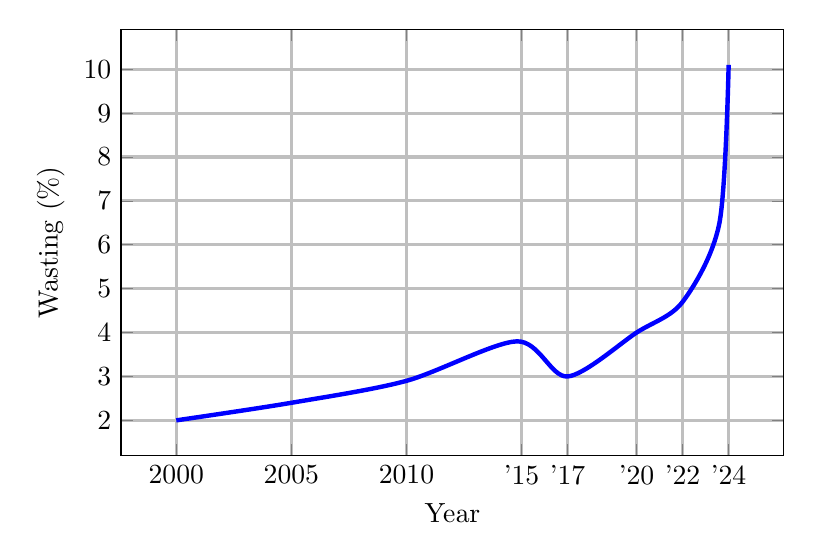
\begin{tikzpicture}
\begin{axis}[
    xlabel={Year},
    ylabel={Wasting (\%)},
    xtick={2000,2005,2010,2015,2017,2020,2022,2024},
    xticklabels={2000,2005,2010,'15,'17,'20,'22,'24},
    ytick={0,1,2,3,4,5,6,7,8,9,10},
    grid=both,
    every axis grid/.append style={line width=0.4mm}, 
    width=10cm,
    height=7cm,
    enlargelimits=true,
    smooth,
    domain=2000:2024
]
\addplot[
    smooth,
    ultra thick,
    blue
] coordinates {
    (2000,2.0)
    (2005,2.4)
    (2010,2.9)
    (2014.8,3.8)
    (2017,3.0)
    (2020,4.0)
    (2022,4.7)
    (2023.6,6.5)
    (2024,10.1)
};
\end{axis}
\end{tikzpicture}
\end{center}

\begin{parts}
\part[3] What was the average rate of change of wasting between 2000 and 2020?
    \vspace{5cm}
\part[3] What was the average rate of change of wasting between 2020 and 2024?
    \vspace{5cm}
\part[2] For what period of time (intervals) is the function \textbf{increasing}? Express your answer in interval notation. 
\end{parts}

\vfill

\newpage

%Ari Davidovsky
\question[8] Solve the given equation: (Hint: check your solutions.)
\[\sqrt{x+7}-x+4=5\]




\end{questions}





\end{document}
